% Chapter 1

\chapter{Introduction} % Main chapter title

\label{Chapter1} % For referencing the chapter elsewhere, use \ref{Chapter1}

%----------------------------------------------------------------------------------------

% Define some commands to keep the formatting separated from the content
\newcommand{\keyword}[1]{\textbf{#1}}
\newcommand{\tabhead}[1]{\textbf{#1}}
\newcommand{\code}[1]{\texttt{#1}}
\newcommand{\file}[1]{\texttt{\bfseries#1}}
\newcommand{\option}[1]{\texttt{\itshape#1}}

%----------------------------------------------------------------------------------------

\section{Project description}
The process of urbanisation has been a double edged sword whereby many a people have benefited from it while a lot more have not. The issue of informal settlements is one that covers areas such socio-economic, governance, climate, politics, healthcare, and resource management to name a few.\\
One of the few approaches to tackle these issues is through good modelling, and understanding the growth of such informal settlements.\\
This project will employ a cellular automata technique, specifically John Conway's 'Game of Life' to model informal settlement growth in South Africa.
\section{Problem description and background}
From the 1950s to the early 2000s the rate of urbanisation has increased 20\%, however the amount of people living in inadequate housing, informal settlements, and slums globally is still about 1 billion.\cite{un}\\
According to the United Nations (UN) the definition of an informal settlement is a dwelling with a lack of security, sanitation, water, living area, and housing durability.\cite{un1} \\
The UN also has a list of 17 Sustainable Development Goals of which number 11 is to create 'Sustainable Cities and Communities'. These goals are such that if even a few can be achieved the other will become easier to achieve as well.
Discuss Informal settlement framework(what, where, when, how of informal settlements)\\\\
Cellular Automata (abbreviated as CA) is a discrete computational model which is studied in automata theory. The basic components of such a model is a grid which contains cells. Each cell can have a finite number of states it can take on. An initial state at time ($t = 0$) is assigned to the grid as a whole. For each time interval thereafter the cells change their states according to a predefined set of rules.\cite{ca}\\\\
Conway's \textit{Game of Life} also known as \textit{Life} was created by the British Mathematician John H Conway in the 1970s and first appeared in the \textit{Scientific American} magazine.\cite{conway}\\
The states the cells in Life can take on are either alive or dead. The rules that govern the states of Life are as follows:
\begin{enumerate}
\item Due to underpopulation a cell will die if it has less than 2 neighbours\footnote{These are cell which are alive and are located around the current cell}.
\item If a cell has 3 or 2 neighbours it will remain alive in the next cycle.
\item If a cell has more than 3 neighbours it will die.
\item If a dead cell is surrounded by 3 alive cells it will become alive in the next cycle.
\end{enumerate}
Using such a set of rules this project will embark on creating a model that will accurately predict informal settlement growth in South Africa.\\
Some limitations have been noted in using CA to model urban growth. These include creating tradeoffs between flexibility and simplicity for the transitional rules. At the same time other opportunities in CA models also present themselves for study such as calibration, stochastic components, and cell types.\cite{ca1}
\section{Aims and objectives}
\subsection{Aims}
\begin{itemize}
\item Create a sound mathematical and statistical model
\item Apply model to Life to predict growth of informal settlements
\end{itemize}
\subsection{Objectives}
\begin{itemize}
\item Conduct the relevant literature reviews
\item Get access to relevant maps needed regarding informal settlements
\item If above step fails, create own maps
\item Create an application that allows a map to be added and a grid to be placed for simulating Life.
\item Create a mathematical and statistical model to provide an initial state
\item Apply initial state to the map
\item Iterate and monitor growth output
\item Calculate accuracy of model by comparing maps from different time periods
\end{itemize}
\section{Procedures and methods}
\subsection{Paradigms}
When a research project is conducted it usually fall under specific paradigms. A research paradigm is defined as "a set of commonly held beliefs and assumptions within a research community about ontological, epistemological, and methodological concerns."\cite{des}\\
The research paradigms are as follows:
\begin{itemize}
\item Positivism
\item Interpretivism
\item Critical realism
\item Critical theory
\end{itemize}
\textit{Positivism} stipulates that reality exists independent of human experiences and actions. It further states that knowledge can be gained from experimentation and observation. Lastly, its strategy focuses on surveys and experiments.\\\\
\textit{Interpretivism} stipulates that a 'social world' is created by humans who conduct social actions and give meaning to the actions. It further states that knowledge can be gained by actively partaking in the phenomenon and the people who create it. Lastly, its strategy focuses on ethnography, action research, and case studies.\\\\
\textit{Critical realism} stipulates that science is not only about observation and there exist mechanisms that are not observable but generate observable behaviours and events. It prefers reduction which is a methodological approach. It begins from unexplained phenomenon and moves to proposing different mechanisms that explain the phenomenon.\\\\
\textit{Critical theory} stipulates that understanding should not be the only goal and human emancipation should be another driving force of research. It strives to expose oppressing effects of political ideologies, cultural practices, and academic theories.\\\\
This project will fall under a combination of Positivism and Interpretivism. The study will be on social factors combined with infrastructure and other related factors that will assist in creating a suitable or viable model.
\subsection{Artefact Life Cycle Philosophies}
When an artefact is developed it can take on different methodologies in its approach. Below is a table that has a few such approaches. The table is a modified example from another source\cite{ieee}.
\begin{table}[H]
\centering
\begin{tabular}{@{}ll@{}}
\toprule
Method                           & Description                                                                                                                                                 \\ \midrule
Crystal Clear                    & Emphasis on 'osmotic communication'                                                                                                                         \\
Disciplined agile delivery (DAD) & Incremental and iterative                                                                                                                                  \\
Extreme Programming (XP)         & Concrete commitments                                                                                                                                        \\
Kanban                           & Incremental improvements                                                                                                                                    \\
Lean Software Development        & Deliver value                                                                                                                                               \\
Scrum                            & Feedback and self management, iterative                                                                                                                     \\
Rational Unified Process (RUP)   & \begin{tabular}[c]{@{}l@{}}Iterative cycles. Each cycle has 4 phases\\Inception, Elaboration, Construction, and Transition.\end{tabular} \\
Waterfall                        & Linear sequential phases                                                                                                                                    \\
Top-down or Bottom-up            & Composition and Decomposition                                                                                                                               \\ \bottomrule
\end{tabular}
\caption{\label{tab:table1}Overview of development methodologies}
\end{table}
\noindent The approach for this project will be Scrum. As it is perfect for incremental changes made to the model that will be created.
\subsection{Collaboration}
A comparative approach will also be taken by integrating work from a fellow student's project. The student will be focusing on CA modelling from a swarm intelligence approach.
\section{Project management}
\subsection{Project Plan}
Self management will be key in this project and all its endeavours.\\
Important dates include:
\begin{itemize}
\item 18 April: Submission of project planning and research proposal
\item 13 June: Submission of literature study          
\item 21 October: Demonstrations of artefact and poster          
\item 1 November: Submission of complete documentation 
\end{itemize}
A basic Gantt chart with overview of the project is shown below
\begin{figure}[H]
\centering
%\includegraphics[width=0.5\textwidth]{spiral}
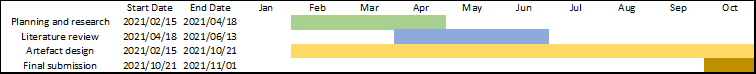
\includegraphics[scale=0.8]{Figures/Chart.png}
\caption{Project plan as represented by a Gantt chart}
\label{fig:fig1}
\end{figure}
\subsection{Scope and Limitations}
The scope for this project is the creating, testing, and computing accuracy of the model. Further research will have to be done in other projects at a later stage. The current limitations for this project is time as the deadline for the final presentations and artefact design is in November 2021. No other limitations with regards to financing or resources exists.\\\\
Risk analysis was conducted and all the risks involved are listed below:
\begin{itemize}
\item Model is not viable
\item Model is not accurate enough
\item Time is not enough to conclude research
\end{itemize}
\section{Development platform, resources, and environments}
Datasets: Still under procurement from third parties (AfriGIS, StatsSA, GeoTerra Image).\\
Operating system: Windows and Linux\\
Programming language: Python will be used\\
IDE: No specific. However current tools include Jupyter Notebooks, Google Colaboratory, and basic text editors.\\
The reason why these tools were chosen is for their versatility, ease of access, plethora of libraries and additional packages that can be imported as needed. 
\section{Ethical and legal implications}
The only legal and ethical implications for this project is in the form of third party data access. The ethics form is attached in Appendix \ref{AppendixA}
\section{Provisional chapter division}
Chapter 1 - Introduction\\
This will cover the outline of the project.\\
Chapter 2 - Literature Review\\
The focus of this section is to delve deeper into the relevant literature for this project and give a thorough analysis.\\
Chapter 3 - Artefact Design\\
The focus of this section will be on the complete processes involved in creating the model for this project.\\
Chapter 4 - Discussion\\
The focus in this section will be to analyse the results gained from the model and compare them to the relevant literature discussed before. Further assumptions and claims are also discussed here. Lastly, comparisons with other students' work will be discussed.\\
Chapter 5 - Conclusion\\
The research project is closed off and further insights for the future can also be given. Aim and objectives are re-examined to ensure if they were achieved.
